\documentclass{article}
\usepackage{parskip}
\usepackage[margin=2cm]{geometry}
\usepackage{graphicx}
\graphicspath{{.}}

% Thanks to Angus Pearson for nagging me to fuck about with fonts in
% XeLaTeX

\usepackage{fontspec} \usepackage{xltxtra}

% PT Serif
\setromanfont[ BoldFont=PTF75F.ttf, ItalicFont=PTZ56F.ttf,
BoldItalicFont=PTF76F.ttf, ]{PTF55F.ttf}

% Noto Sans
\setsansfont[ BoldFont=NotoSans-Bold.ttf,
ItalicFont=NotoSans-Italic.ttf, BoldItalicFont=NotoSans-BoldItalic.ttf
]{NotoSans-Regular.ttf}

\begin{document}

\textbf{\Huge Operating Systems Notes}

\section{OSs and Architectures}

Different architectures dictates the way that an operating system must conduct its business.

As different architecture platforms have different instruction sets, it determines what are viable methods for accomplishing tasks such as \textit{memory protection} and \textit{control interrupts}.

\subsection{Privileged Instructions}

These instructions are restricted to use by the OS \textit{only}, and includes direct access to \textit{I/O devices} and \textit{memory state management}.

This is achieved by the implementation of two \textit{modes of operation}; \textit{user} and \textit{kernel} modes.
\begin{figure}[h!]
  \centering
  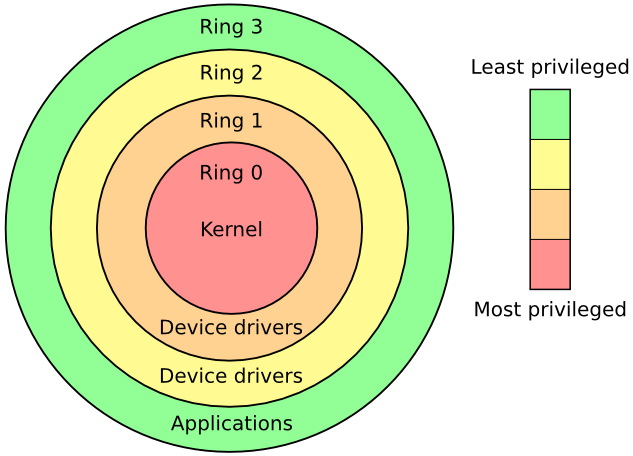
\includegraphics[scale=0.35]{privilegeGraphX86}
  \caption{x86 Architecture Levels of Privilege}
  \textit{Courtesy of Hertzsprung of English Wikipedia}
\end{figure}

More words?

\end{document}